\documentclass[11pt]{article}
\usepackage[letterpaper,margin=.72in]{geometry}
\usepackage[T1]{fontenc}
\usepackage{lmodern,microtype,graphicx,booktabs,amsmath,hyperref}
\usepackage{xurl}
\hypersetup{colorlinks=true,urlcolor=blue,pdfauthor={James N. Jean IV},pdftitle={Cancellation-aware airport reliability}}
\setlength{\parindent}{0pt}\setlength{\parskip}{6pt}\renewcommand{\arraystretch}{1.1}
\begin{document}
{\Large\bfseries Cancellation-aware airport reliability}\par
James N. Jean IV\hfill 29 October 2026\par
\textit{Independent study 03. Not peer reviewed.}
\section*{Decision brief}
Which denominator should a reliability display use when some scheduled flights do not reach their destination? This finite comparison separates a constructed completed-flight on-time rate from an all-scheduled-flight rate, using a fixed 2019 airport reference mix.

A constructed completed-flight view raises the fixed-airport-weight on-time percentage by 0.708--1.353 percentage points across the six prespecified UA/WN carrier-year panels in 2023--2025. These are the same captured count cells with different denominators. The official BTS tabular on-time percentage already uses scheduled totals; this is not evidence that BTS omits cancellations.

Display scheduled-flight on-time, cancelled and diverted shares together, with the exact denominator and airport coverage. A completed-flight view can be a supplementary diagnostic. Verify reporting scope and original dated inputs before using these comparisons for a service decision; passenger-delay or rebooking decisions require passenger data.

\begin{center}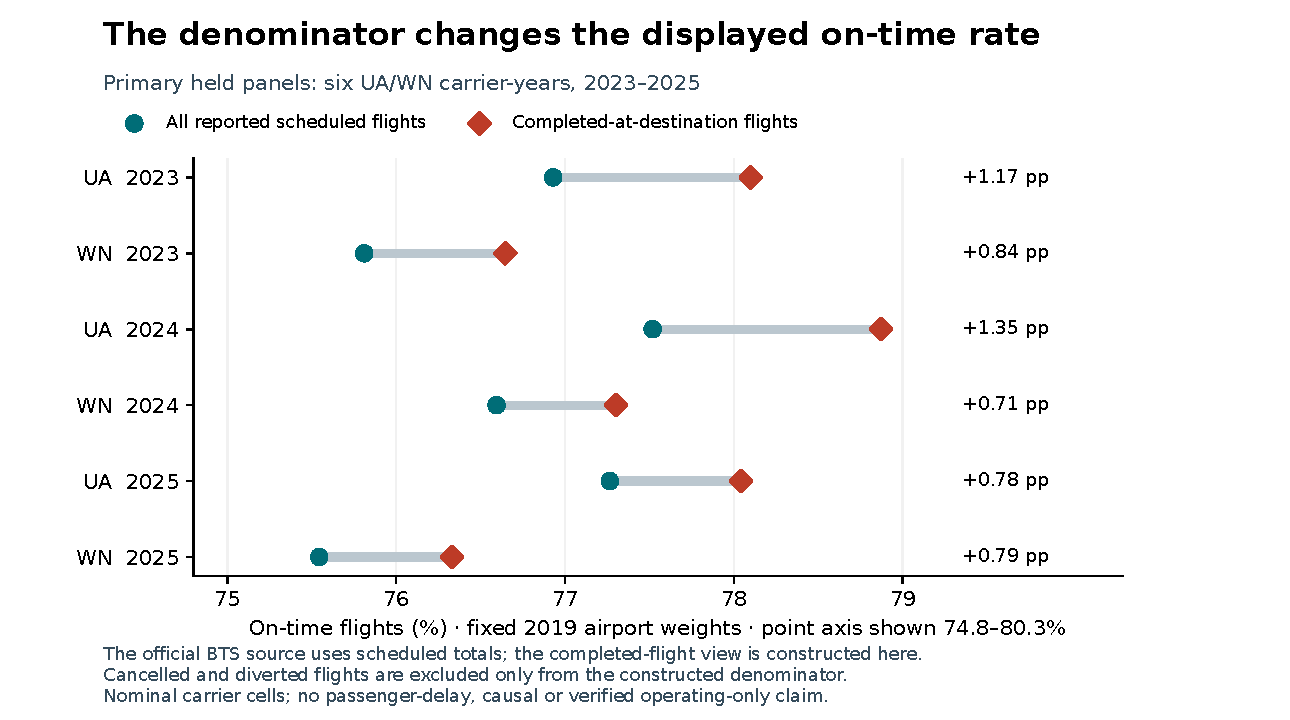
\includegraphics[width=\linewidth]{images/denominator_rates.pdf}\end{center}
\small Figure 1. All six primary held panels. The completed-flight metric is constructed in this study; the official source uses scheduled totals. Point-axis limits are stated explicitly. These rates describe count cells, not passenger arrivals.\normalsize\par

\newpage\section*{1. Source, scope and fixed design}
The official BTS form export [1] covers January 2019--December 2025. Its 6,095,050-byte ZIP contains 161,415 airport/carrier/month rows. Analysis publishes only eight factual key/count fields for AA, DL, UA and WN: 38,069 rows. Source, member and projection hashes are retained. Independent standard-CSV and pandas C-parser projections match 1,291,320 scalars across the complete file; four exact count and four rounded-percentage controls match a separately requested official tabular view.

The source has no operating-versus-marketing flag. Treat these as nominal carrier-code count cells, not independently verified operating-only or disjoint populations [2,3]. The reference weights are a function of published cells and are not asserted unique-flight market shares. Original historical publication vintages, complete schedule coverage and source truth remain unknown. Raw archives, full reports, flight/customer/tail identifiers and third-party prose stay outside GitHub. The public scope is minimal factual counts with attribution and original work [6,7], not a source-wide license claim.

The initial cohort contains all 58 airports with twelve valid positive-total entries in 2019 for each of the four fixed codes. Each carrier-year retains baseline airports with twelve valid positive-total monthly cells. Preserve all exclusions and baseline reference-volume coverage. Null/absent entries are not zero or verified service exit. Baseline weights pool reported 2019 count cells across the four codes, then renormalize on each complete-year panel. This controls recorded airport mix only.

\begin{center}\small\setlength{\tabcolsep}{4pt}
\begin{tabular}{lll}\toprule
Symbol & Meaning & Rate denominator \\
\midrule
N & Reported scheduled-total count & N \\
D & Arrival delay at least 15 minutes & N or B \\
C & Cancelled count & N \\
V & Diverted count & N \\
O & Residual on time: N-D-C-V & N or B \\
B & Completed at destination: N-C-V & B \\
Gap & O/B minus O/N & Percentage points \\
\bottomrule\end{tabular}\end{center}
AA/DL in 2020--2022 are development carriers/years; the six primary held panels are UA/WN in 2023--2025. All remaining fixed carrier-years are retained as secondary descriptions. Baseline inputs include all four codes, so this is not unseen-carrier prediction. Source quality and inputs were visible without blinding. Twenty-five analytical dependencies were frozen at 5f23c46 before held summaries; no fitting, model selection, optimizer or survival model is used.

\newpage\section*{2. Primary denominator comparison}
All rates below use the same fixed airport reference weights. Completed and scheduled on-time percentages differ only in whether cancelled/diverted flights remain in the denominator. The gap is in percentage points, not percent change. Reported N is the pooled cell-count total inside that carrier-year panel, not a passenger total or independently verified unique-flight population.

\begin{center}\small\setlength{\tabcolsep}{4pt}
\begin{tabular}{lrrrrrrr}\toprule
Code & Year & Reported N & Completed & Scheduled & Gap pp & Cancel & Divert \\
\midrule
UA & 2023 & 444,416 & 78.100 & 76.930 & 1.170 & 1.280 & 0.225 \\
WN & 2023 & 1,005,692 & 76.646 & 75.811 & 0.835 & 0.918 & 0.175 \\
UA & 2024 & 464,998 & 78.871 & 77.519 & 1.353 & 1.487 & 0.225 \\
WN & 2024 & 1,005,250 & 77.303 & 76.594 & 0.708 & 0.730 & 0.181 \\
UA & 2025 & 487,337 & 78.042 & 77.265 & 0.776 & 0.748 & 0.252 \\
WN & 2025 & 999,900 & 76.331 & 75.545 & 0.786 & 0.826 & 0.201 \\
\bottomrule\end{tabular}\end{center}
\small Rates other than N and the gap are percentages. Every primary panel uses all 58 baseline airports.\normalsize\par

For a nonnegative partition with N>0 and B>0, the gap is algebraically determined:

\[\frac{O}{B}-\frac{O}{N}=\frac{O(C+V)}{NB}\geq0.\]
The nonnegative difference is a mathematical identity, not a newly discovered causal effect or evidence of manipulation. Its finite magnitude depends on the observed count cells and chosen reference weights. The official BTS source already retains cancellations and diversions in its displayed scheduled denominator. The constructed completed-flight metric asks a different conditional question.

Annual counts sum monthly cells before each airport rate is calculated. Monthly results are also retained for all 72 primary carrier-months, all other held panels and every synthetic conversion. A standardized conditional summary would be undefined if any positive-weight airport had a zero completed denominator; no such airport is silently dropped. The executed weighted panels have no undefined metric rows, while the fixtures exercise that boundary explicitly.

Display scheduled-flight on-time, cancelled and diverted shares together, with the exact denominator and airport coverage. A completed-flight view can be a supplementary diagnostic. Verify reporting scope and original dated inputs before using these comparisons for a service decision; passenger-delay or rebooking decisions require passenger data.

This is a retrospective descriptive calculation on nominal published carrier codes, not independently verified operating-only or disjoint populations. Fixed airport weights do not control routes, weather, season or passengers. No causal airline strategy, actual cancellation action, passenger benefit, novelty or future performance is established.

\newpage\section*{3. Airport mix and retained coverage}
Observed-pool and fixed-airport-weight scheduled on-time percentages below use identical count cells within each carrier-year. Their difference describes these aggregation choices, not an airport effect or airline ranking under equal routes. AA/DL are prespecified secondary held-year descriptions.

\begin{center}\small\setlength{\tabcolsep}{4pt}
\begin{tabular}{lrrrrrr}\toprule
Code & Year & Airports & Weight \% & Pooled \% & Fixed \% & Diff pp \\
\midrule
AA & 2023 & 58 & 100.000 & 75.761 & 73.856 & 1.905 \\
DL & 2023 & 58 & 100.000 & 83.053 & 81.865 & 1.188 \\
UA & 2023 & 58 & 100.000 & 78.063 & 76.930 & 1.133 \\
WN & 2023 & 58 & 100.000 & 76.764 & 75.811 & 0.953 \\
AA & 2024 & 58 & 100.000 & 72.474 & 70.184 & 2.290 \\
DL & 2024 & 58 & 100.000 & 82.139 & 80.875 & 1.264 \\
UA & 2024 & 58 & 100.000 & 78.572 & 77.519 & 1.053 \\
WN & 2024 & 58 & 100.000 & 78.271 & 76.594 & 1.677 \\
AA & 2025 & 57 & 99.862 & 73.323 & 70.703 & 2.620 \\
DL & 2025 & 58 & 100.000 & 79.679 & 78.006 & 1.673 \\
UA & 2025 & 58 & 100.000 & 78.276 & 77.265 & 1.010 \\
WN & 2025 & 58 & 100.000 & 77.185 & 75.545 & 1.640 \\
\bottomrule\end{tabular}\end{center}
\begin{center}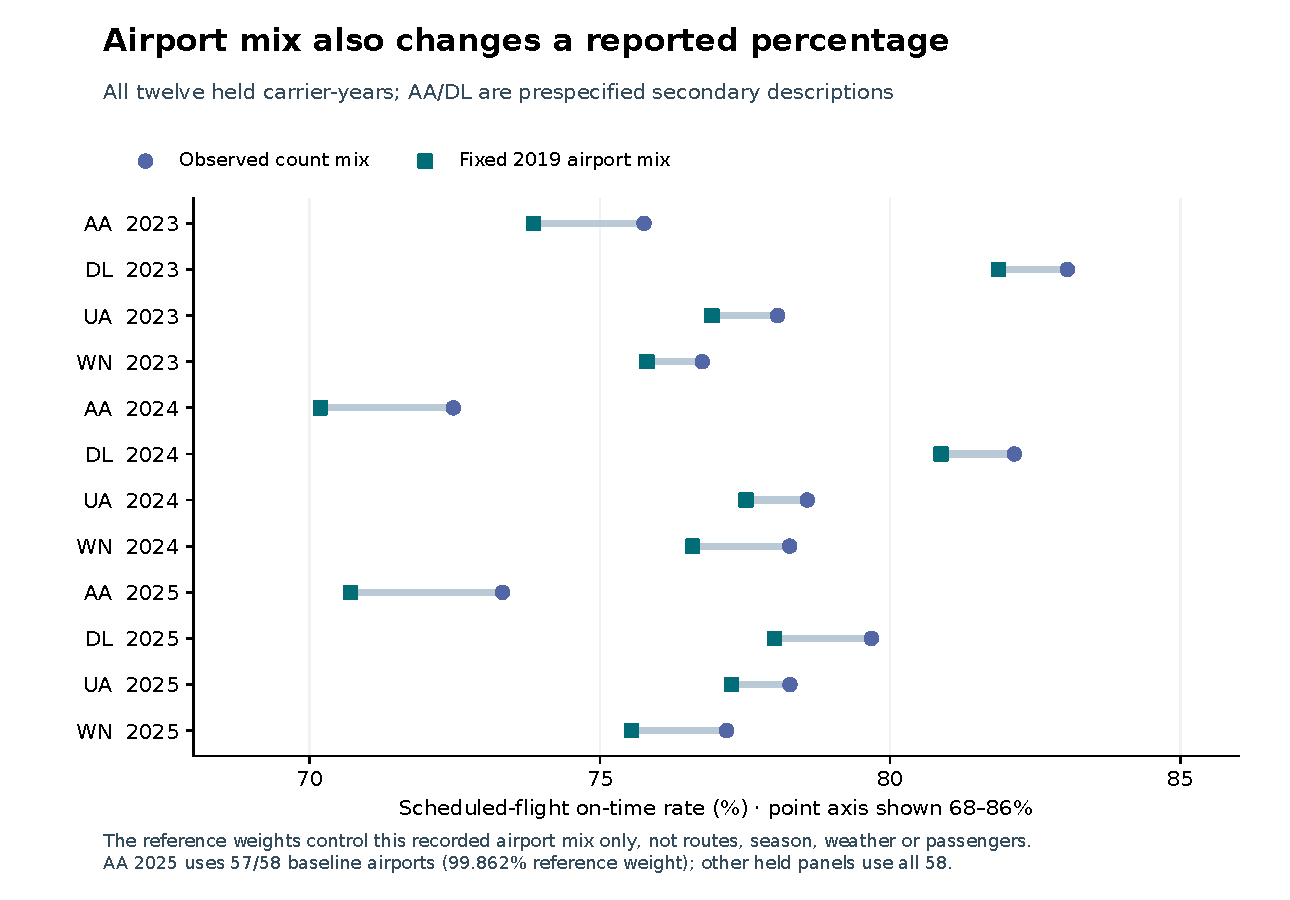
\includegraphics[width=.88\linewidth]{images/airport_mix.pdf}\end{center}
\small Figure 2. Every held carrier-year is shown. AA 2025 omits one baseline airport and retains 99.862\% of reference weight; other held panels retain all 58. The complete-case benchmark can miss entering, incomplete or differently served airports.\normalsize\par

\newpage\section*{4. Complete synthetic conversion grid}
At each monthly carrier-airport cell, convert floor(q times D) delayed counts to cancelled counts for all fixed q values: 0, 10\%, 25\% and 50\%. Keep N, V and O unchanged. The zero setting is the identity. The table reports increases in the standardized completed-flight on-time rate; the scheduled-flight rate change at 50\% is exactly zero. The same invariance holds at every conversion setting.

\begin{center}\small\setlength{\tabcolsep}{4pt}
\begin{tabular}{lrrrrr}\toprule
Code & Year & 10\% gain pp & 25\% gain pp & 50\% gain pp & Scheduled change \\
\midrule
AA & 2023 & 1.859 & 4.956 & 10.722 & 0.000 \\
DL & 2023 & 1.381 & 3.644 & 7.712 & 0.000 \\
UA & 2023 & 1.652 & 4.427 & 9.524 & 0.000 \\
WN & 2023 & 1.782 & 4.691 & 10.064 & 0.000 \\
AA & 2024 & 2.030 & 5.412 & 11.825 & 0.000 \\
DL & 2024 & 1.454 & 3.839 & 8.143 & 0.000 \\
UA & 2024 & 1.614 & 4.307 & 9.236 & 0.000 \\
WN & 2024 & 1.730 & 4.559 & 9.780 & 0.000 \\
AA & 2025 & 1.996 & 5.316 & 11.593 & 0.000 \\
DL & 2025 & 1.627 & 4.299 & 9.193 & 0.000 \\
UA & 2025 & 1.660 & 4.440 & 9.537 & 0.000 \\
WN & 2025 & 1.794 & 4.730 & 10.160 & 0.000 \\
\bottomrule\end{tabular}\end{center}
\begin{center}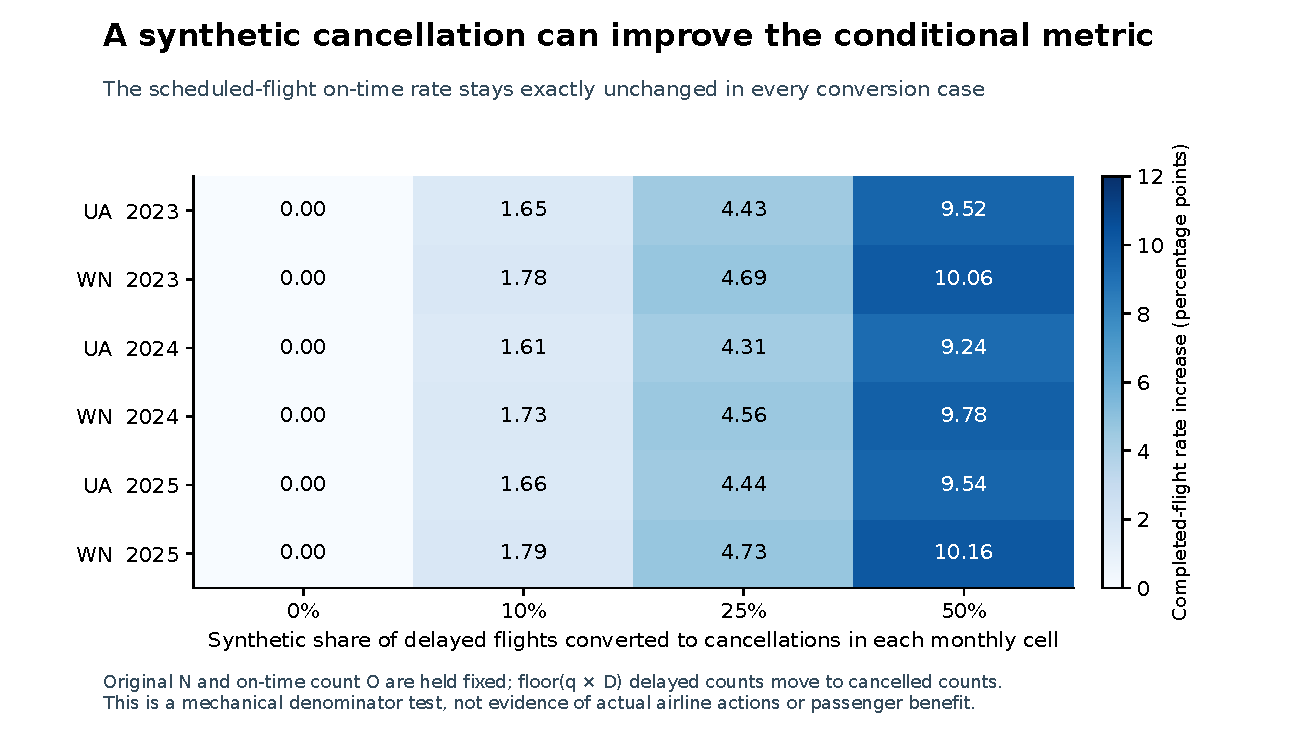
\includegraphics[width=.92\linewidth]{images/synthetic_conversion.pdf}\end{center}
\small Figure 3. All six primary panels and all four conversion fractions. The larger conditional percentage does not represent an extra on-time flight. Fractions are untuned stress assumptions, not estimated airline behavior.\normalsize\par

\newpage\section*{5. Development, failures and independent checks}
The complete baseline/development panel summaries are retained below. UA/WN development-year rows are secondary descriptions; no fitting or parameter selection occurs. The source benchmark is retrospective and revised-publication availability is not a passed prospective gate.

\begin{center}\small\setlength{\tabcolsep}{4pt}
\begin{tabular}{lrrrrrr}\toprule
Code & Year & Airports & Weight \% & Completed \% & Scheduled \% & Gap pp \\
\midrule
AA & 2019 & 58 & 100.000 & 77.144 & 75.469 & 1.675 \\
DL & 2019 & 58 & 100.000 & 85.062 & 84.764 & 0.297 \\
UA & 2019 & 58 & 100.000 & 77.930 & 77.140 & 0.790 \\
WN & 2019 & 58 & 100.000 & 81.191 & 79.092 & 2.099 \\
AA & 2020 & 48 & 96.515 & 88.254 & 82.920 & 5.334 \\
DL & 2020 & 52 & 97.896 & 90.401 & 85.745 & 4.656 \\
UA & 2020 & 33 & 75.313 & 89.852 & 82.999 & 6.853 \\
WN & 2020 & 58 & 100.000 & 93.279 & 85.566 & 7.713 \\
AA & 2021 & 51 & 96.722 & 81.288 & 79.402 & 1.886 \\
DL & 2021 & 54 & 99.113 & 87.910 & 87.310 & 0.601 \\
UA & 2021 & 49 & 94.878 & 81.021 & 79.780 & 1.241 \\
WN & 2021 & 58 & 100.000 & 77.128 & 75.447 & 1.680 \\
AA & 2022 & 57 & 99.735 & 75.378 & 73.211 & 2.167 \\
DL & 2022 & 58 & 100.000 & 83.568 & 82.137 & 1.431 \\
UA & 2022 & 57 & 96.040 & 79.585 & 78.014 & 1.571 \\
WN & 2022 & 58 & 100.000 & 74.437 & 71.841 & 2.596 \\
\bottomrule\end{tabular}\end{center}
Independent verification reconstructs cohorts, complete-year panels, baseline weights and every transformed count using SQLite, then reconstructs each metric with exact rational arithmetic without importing model helpers. Development checks cover 865,095 exact exported fields and 168,675 conversion-identity checks; held checks cover 725,563 fields and 135,525 identities. Fifteen hand-calculated/boundary fixtures pass. Isolated replay matches 1,399,126 exact CSV fields plus four summary/verification documents and all 25 protected dependencies.

The initial source projection stopped on 243 positive-total cells with a blank delay count, including 23 selected cells. An independent parser confirmed N=C+V in every such case: nonnegative D+O=N-C-V=0 uniquely identifies derived D=O=0. Original blanks remain blank, logical resolution is labelled, and conditional B=0 rates stay undefined. Another 294 source rows (42 selected) have unknown totals and remain unknown; their cells cannot pass complete-year eligibility. The original failed receipt is retained. A later null-diagnostic coding error stopped after controls but before the manifest and was repaired without changing projected source values.

Three original figures pass 168 actual artist-value checks, six gap annotations, 24 heatmap labels/contrast checks and nine export hashes. Initial legend/footer overlaps were repaired; failed figures remain private. Figure checks and page inspection are finite evidence, not accessibility conformance. The first figure-checker expression used a Python syntax unavailable in 3.10; its targeted correction changes no data or analysis.

\newpage\section*{6. Interpretation, next evidence and sources}
The practical decision is to show both the service outcome and its conditioning population. Scheduled on-time, cancellation and diversion shares preserve the scheduled denominator. Completed-flight delay or punctuality can support a separate operational diagnostic when explicitly labelled. Neither view alone measures passenger delay, rebooking, connections, satisfaction, capacity, actual unserved demand or welfare.

Fixed 2019 weights remove one recorded airport-mix difference; they do not equalize origin-destination routes, seasonal schedules, aircraft, weather or passenger loads. Complete-year eligibility selects a published-data benchmark, and a small excluded weight does not validate missing cells. Source carrier reporting identity and historical vintages remain qualified. The primary held-year comparison is an audit of fixed descriptive calculations, not forecasting or a guarantee about future service.

Before an operational comparison, obtain dated reporting snapshots, authoritative carrier/network scope and schedule coverage, then prospectively specify route/season controls. Passenger claims require itinerary, load, connection and rebooking evidence with appropriate privacy protection. Such extensions require a new protocol; they are not implied by this monthly export.

Prior work already identifies the limits of flight-based punctuality for passenger delay [4] and studies cancellation choices and delay forecasts [5]. This study offers a transparent finite count/denominator reconstruction with explicit source-null and population accounting. It introduces no new estimator, exhaustive literature gap or demonstrated operational benefit. The broader proposal's weather adjustment, route standardization and survival-analysis claims are outside this scoped release.

\small
1. BTS, official delay-cause form and download\par\url{https://www.transtats.bts.gov/ot_delay/OT_DelayCause1.asp}\par
2. BTS, reporting and delay definitions\par\url{https://www.bts.gov/topics/airlines-and-airports/understanding-reporting-causes-flight-delays-and-cancellations}\par
3. BTS, carrier/reporting scope and on-time definitions\par\url{https://www.bts.gov/explore-topics-and-geography/topics/airline-time-performance-and-causes-flight-delays}\par
4. Bratu and Barnhart, An Analysis of Passenger Delays Using Flight Operations and Passenger Booking Data\par\url{https://doi.org/10.2514/atcq.13.1.1}\par
5. Seelhorst (2014), Flight Cancellation Behavior and Aviation System Performance\par\url{https://escholarship.org/uc/item/3045w49k}\par
6. U.S. Copyright Office, facts versus protected expression\par\url{https://www.copyright.gov/help/faq/faq-protect.html}\par
7. DOT National Transportation Library, Licensing for Data\par\url{https://rosap.ntl.bts.gov/view/dot/77432}\par
\normalsize\par
Reproduction: install pinned requirements; run the fifteen fixtures, isolated replay, figure/paper checks and canonical package verification. Source/protocol history, all results, failed source receipt and exclusions remain inspectable in the repository. Reviewed independent manuscripts are public after checks; Azure optimization and other formal-publication projects remain private.

\end{document}
